\documentclass[10pt,aps,pra]{revtex4-1}

\usepackage[utf8x]{inputenc}
\usepackage[english,russian]{babel}

\usepackage{amsmath}
\usepackage{graphicx}
\usepackage{verbatim}
\usepackage{color}
\usepackage{subfigure}
\usepackage{hyperref}
\usepackage{float}

\usepackage[mathlines]{lineno}


\setcounter{figure}{0}
\raggedbottom

\begin{comment}
\pagestyle{empty}
\end{comment}

\begin{document}

\title{Модель complex networks withpicky}Snarskii}KPI}{IPRI}%{89.75.Hc}trees}%{02.10.Ox}
author  Igor,  \{NTUU\ \ {Networks\ {Combinatorics;
\{Zarvanskiy  affiliation
affiliation

and genealogical pacs
pacs graphtheory}%{89.75.-k}systems}%{05.10.-a}dynamics}
{Complex  \ pacs \{May
pacs  {Computationalmethods in statistical physics and nonlinear

\date  01, {abstract}

2014}\ begin
In this article considered a model ... and its difference; model ... are ...

First, consider the model of connecting with m. n. picky, communication and unlike the model Barabasi-Albert. Next, we consider the model (u, v) -flowers, the results of numerical simulation and study the various characteristics of the growing (u, v) -flowers when connecting with picky. And in this case, the numerical simulation leads to the phenomena of the same phase transitions of the second kind.
End  \\\\{Introduction}
\maketitle

linenumberspar

{abstract}section

A large number of real complex networks are scale-free networks, such degrees are distributed according to a power law. These networks include the WWW-networks, metabolism, power supply (food webs), social networking and many other \ cite {Dor2}.

Currently, the properties of such scale-free networks have been studied, established their network characteristics (average degree of a node, the minimum middle path, clustering coefficient, etc.) \ cite {Newman}. It should be noted that the complex network scenarios constructed under the assumption \ cite {AlBa2} is an idealization of real networks, the characteristics of which can sometimes differ significantly from the ideal \ cite {Newman}. Nevertheless, the power law degree nodes of real complex networks is quite common, especially for those networks that are formed (perhaps most organized) developing time process \ cite {}.

One such process, which has been studied long before the concept of a complex network, was the distribution process between people "wealth" (by which you can understand money, investments, real estate ...). In \ cite {Pareto} Pareto was set t. N. Pareto's law - the degree of wealth distribution - when the number of people $ \ nu $, vldeyuschih $ \ mu $ - share of wealth is a power function $ \ nu \ sim \ mu ^ \ gamma $, with $ \ gamma = ... $ turns that 20 \% of the people own 80 \% bogastva what is often called the law 80/20.

The paper \ cite {AlBa1} was found scenario of a complex network, ie. n. scenario Barabasi-Albert power-law degree distribution of nodes, based on two fundamentally important provisions:
begin {enumerate} \
\item The network is growing, starting with some of the seed number of nodes $ m_0 $, at each time step there is a certain number of new nodes with $ n $ connections.
\ item The probability of connection links from the new node to the existing ones is directly proportional to the degree.
\ end {enumerate}
In short Barabasi-Albert model - a growing network to the preferred connection.

Subsequently, there are many versions of the algorithm Barabasi-Albert in \ cite {AlBa2} their lists about 20. They all lead to the scaleless networks with different values ​​of the exponent of the distribution of nodes in their powers. At first glance, it appears that a growing network with different types of preferred connection is required to grow in scale-free network.

Shown in this paper that there may be such a minor at first glance, the modification of the law of the preferred compounds in which a power-law distribution model Barabasi-Albert fundamentally broken. In the distribution function at the same time there is a failure, indicating the absence of nodes in the network for a range of values ​​of the degree. As shown by detailed studies, the input parameter $ r $, which determines the modification of the law of the preferred connection has a threshold value $ r_c $, so that when $ r <r_c $ bezmashtabnoy network is a network, and if $ r \ geq r_c $ dip appears. The magnitude of the failure of a power depends on the proximity parameter $ r $ to its threshold value, which suggests an analogy with the second order phase transition.

Modification Law connection has also been tested by us on the hierarchical scale-free networks of deterministic, ie. N. determanirovanyh (u, v) -flowers \ cite {Dor1}. In this case also there was a violation of the power distribution function is similar to the laws of the phase of the second kind.


\ Section {Model Barabasi-Albert with pridirchiostyu}
\ subsection {Algorithm Barabasi-Albert}
Consider the growing network. The standard model of Barabasi-Albert \ cite {AlBa1} at the first time step, there is a $ m_0 $ nodes interconnected. At each step there is a new $ m $ nodes with $ q $ bonds. $ P_i $ - probability of connection (creating links between nodes) of a new node to an existing node $ i $ is proportional to the degree (number of links a node $ i $) - $  $:{k_i}

begin \ {
k_i\{equation}p_i =frac sum \ limits_  k_j}, \{equation}
\{j}end
where the summation is over all the "old" nodes.

Such an algorithm, a large number of time steps leads to a power function of the degree distribution $ P (k) $:

\ begin {  label  powerlaw}\{-\  \{equation}
equation} \{eq:P (k)sim k ^ gamma},
end
with exponent $ \ gamma = 3 $ \ cite {AlBa1}.

In \ cite {AlBa2} contains many modifications to the rules of the preferred connections that lead to different values ​​of the exponent $ \ gamma $. However, the very power dependence of \ eqref {eq: powerlaw} remains.

\ Subsection {Modified Algorithm Barabasi-Albert}
Here we propose a generalization of the model based on the rule of the preferred compounds introduced Barabasi-Albert. The new rule of preference for brevity call connection with `captiousness '' (exceptive). According to this model, a new parameter exceptive - $ r $, taking values ​​in the range of $ (0, 1) $. In the case where the choice of connecting new bond fell to a node $ i $ to the degree of $ k_i $, connection occurs with probability $ p_i $, but only if the following condition {eq:

holds:\ begin {equation} \ label  exceptive {k_i}{j} k_j},{equation}
p_i =  frac  {\ sum \ limits_  \ quad k_i \ geq r \ langle k \ rangle, \
}\end
where $ \ langle k \ rangle $ - average value of the degree of the nodes in the network at the time of accession, $ \ langle k \ rangle = \ sum \ limits_ {j} {k_j} / {N} $.

introducing additional conditions \ eqref {eq: exceptive} pattern during network growth truncates the node (making them as invalid) , ie it is currently unable to join a new connection. It should be noted that if at a given time a node does not satisfy the condition \ eqref {eq: exceptive}, it does not mean that at the following times to it will not be able to join the new nodes. Validity or invalidity in the node changes over time, as changes over time, the value of $  langle k \ rangle $. \

\Subsection {The distribution function of the degrees of nodes}
When the value of fault-finding $ r = 0 $, the proposed model into the standard model of Barabasi-Albert. What is surprising is the presence of a threshold parameter faultfinding $ r_c $. When the parameter is less than a certain threshold faultfinding $ r_c $, ie when $ r <r_c $ node degree distribution function $ P (k) $ is a power, and the network itself, thus, scale-free network. When values ​​of fault-finding larger than the threshold $ r \ geq r_c $ network changes its structure, namely the network nodes disappear from the "average" number of connections that we can see in Fig. \ Ref {fig: rankDistribution_rank}.

Define the threshold value of the fault-finding. To calculate this threshold value for the network nodes 100, and then to step 100 knots will increase the size of the network node 2000, and the values ​​will be averaged for 10 experiments. For a network of 100 nodes $ r_c = 0.62 $, more saturation occurs $ r_c $. For a network of 1,100 nodes $ r_c $ is completely saturated and we get $ r_c = 0.51 $. In the following calculations we will use $r_c=0.51$.


\begin{figure}[H]  

\centering
\subfigure[]
{
    \label{fig:rankDistribution_rank}
    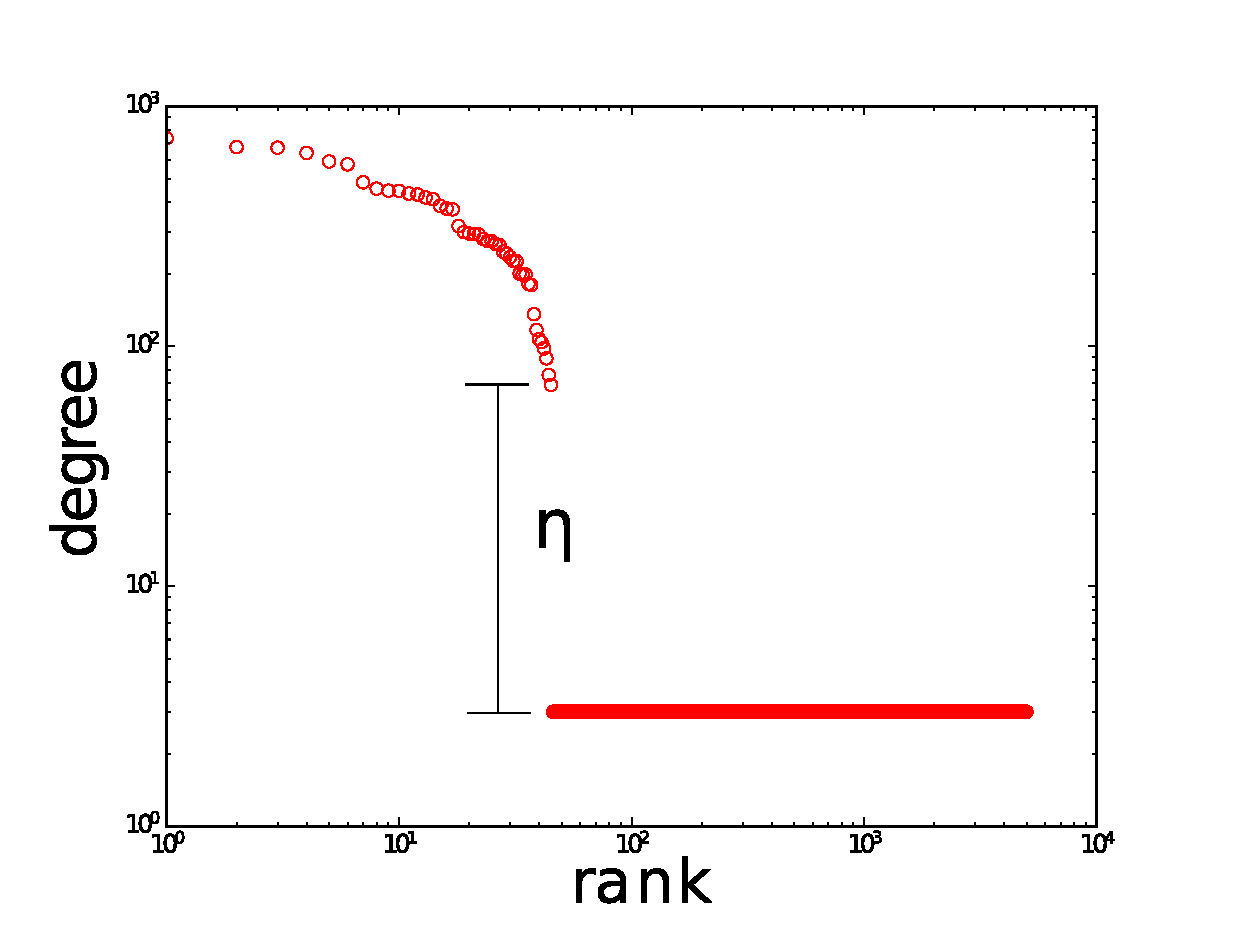
\includegraphics[height=5.5cm]{pygraph/baRank.eps}  
}  
\subfigure[]
{
    \label{fig:rankDistribution_gap}
    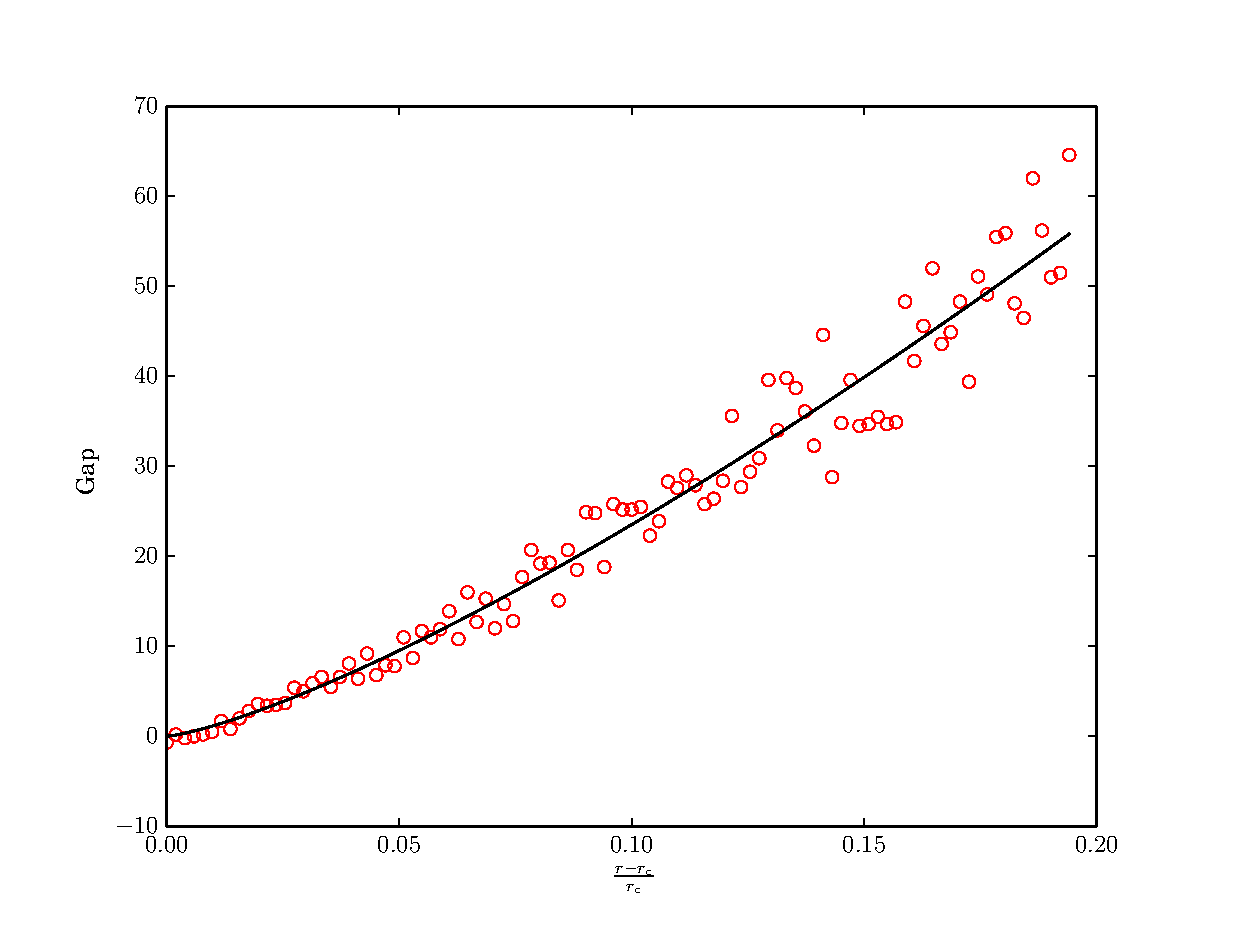
\includegraphics[height=5.5cm]{pygraph/baGap.eps}
}

\caption{
\label{fig:rankDistribution}
\subref{fig:rankDistribution_rank} Ranking distribution network when $ r = 0.6 $. The horizontal axis represents the serial number of the site, the vertical axis is the degree of the node.
\ Subref {fig: rankDistribution_gap} The magnitude of the gap with increasing $ r $ from $ r_c $ to $ r_c + 0.01 $ increments $ 0.001 $. The horizontal axis is $ \ frac {r-r_c} {r_c} $, the vertical axis represents the value of the
gap.}{figure}
\ End


We introduce a new characterization of the network - the magnitude of the gap $ \ eta $ Fig. \ Ref {fig: rankDistribution_rank}, the distance between the nodes closest to the rupture (the difference between the values ​​of the degree of a node before the break and after the break). Size of the gap, the vertical axis indicates the values ​​of the degrees of the nodes that are missing.

According to the numerical simulation of the behavior of the parameter $ \ eta $ is similar to the behavior of the order parameter in the theory of phase transitions of the second kind of \ cite {Landau}. As is known, the order parameter $ \ eta $, for example magnetization as the temperature approaches the critical value of $ T_c $ decreases power law $ \ eta \ sim (r-r_c) ^ \ beta $, where $ \ beta $ - critical index.
When The numerical experiments were selected following initial parameters: the number of nodes $ N = 5000 $, the initial number of nodes $ m_0 = $ 20, the number of connections for each new node $ m = 3 $.

Fig. \ Ref {fig: rankDistribution_gap} obtained dependence $ \ eta = A \ cdot {(r-r_c)} ^ \ beta $, where $  beta \ sim 1.3 $ \

\subsection {Coefficient of clustering, assortative, the minimum average distance, the value of break}
The appearance of the gap $ \ eta $ in the distribution of degrees of nodes $ P (k) $ indicates a significant change in the structure of the network, which can not but affect its performance. The following describes the behavior of $ C $ - clustering coefficient, $ A $ - assortative and $ l $ - minimum average distance as a function of the coefficient of faultfinding $ r $, with $ r \ geq r_c $. As shown by numerical experiment for a network with $ N = 5000 $ node clustering coefficient $ C $, assortative $ A $, the minimum average distance $ l $ with $ r <r_c $ from $ r $ is independent and is equal to $ C_0 \ approx 0.01 $, $ l_0 \ approx 3.98 $, $ A_0 \ approx -0.096 $, that is as it should be, the same as the calculations given in \ cite {AlBa2, Newman2}.

With increasing $ r $ from $ r_c $ to $ r_c + $ 0.01 in increments of $ 0.001 $ clustering coefficient increases from $ 0.04 $ to $ 0.14 $ assortative decreases from $ -0.3 $ to $ -0.6 $, the average minimum distance is reduced from $ 3.5 $ to $ 2.9 $ (as shown in Fig. \ ref {fig: baCharacteristic_raw} ). To normalize the parameter dependence we take the relation to its value at $ r <r_c $, and give according to an increasing function: $ A = \ frac {A} {A_0} $, $ C = \ frac {C} {C_0} $, $l=-\frac{l}{l_0}$.

\begin{figure}[H]  

\centering
\subfigure[]
{
    \label{fig:baCharacteristic_raw}
    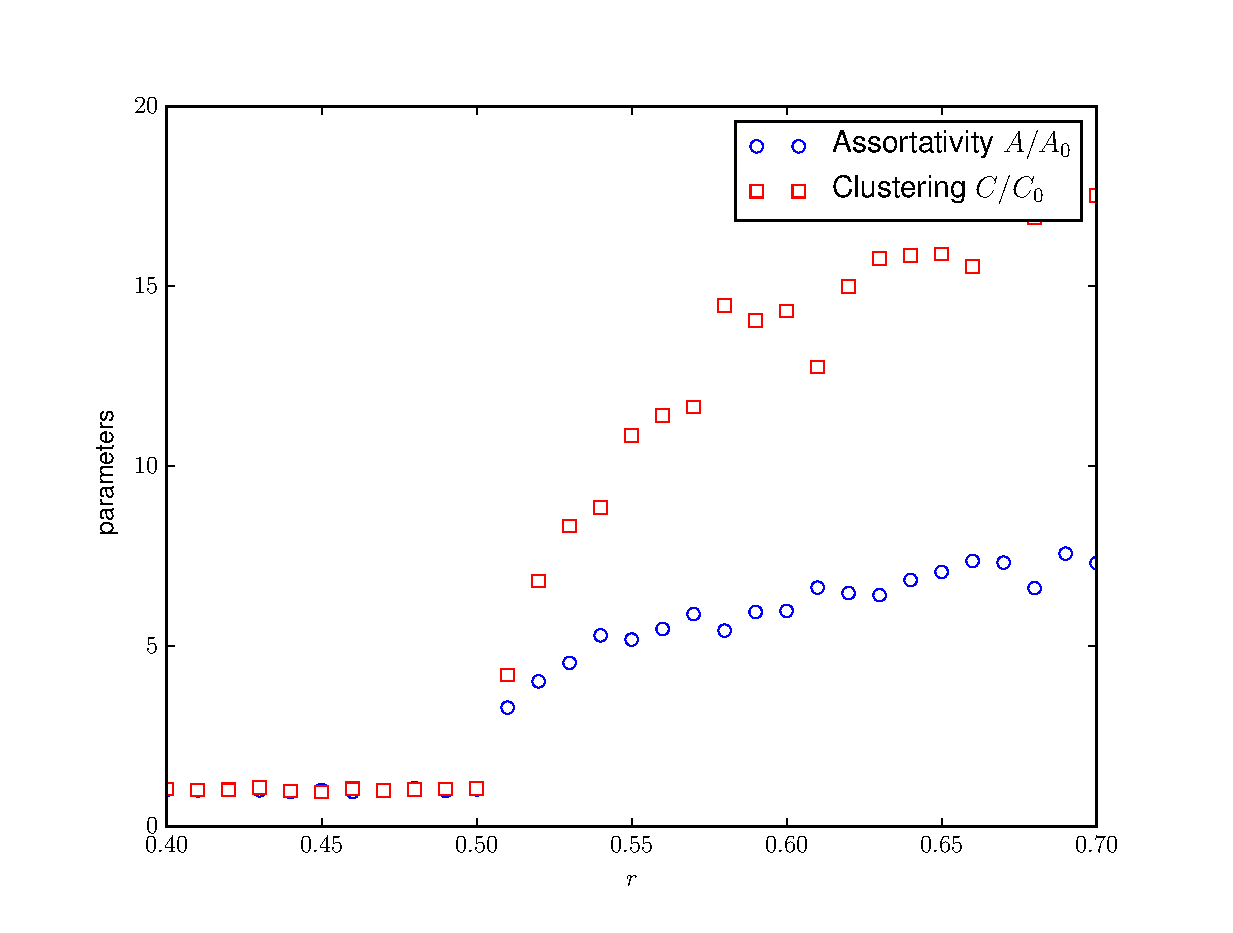
\includegraphics[height=5.5cm]{pygraph/baParams.eps}
}  
\subfigure[]
{
    \label{fig:rankDistribution_log}
    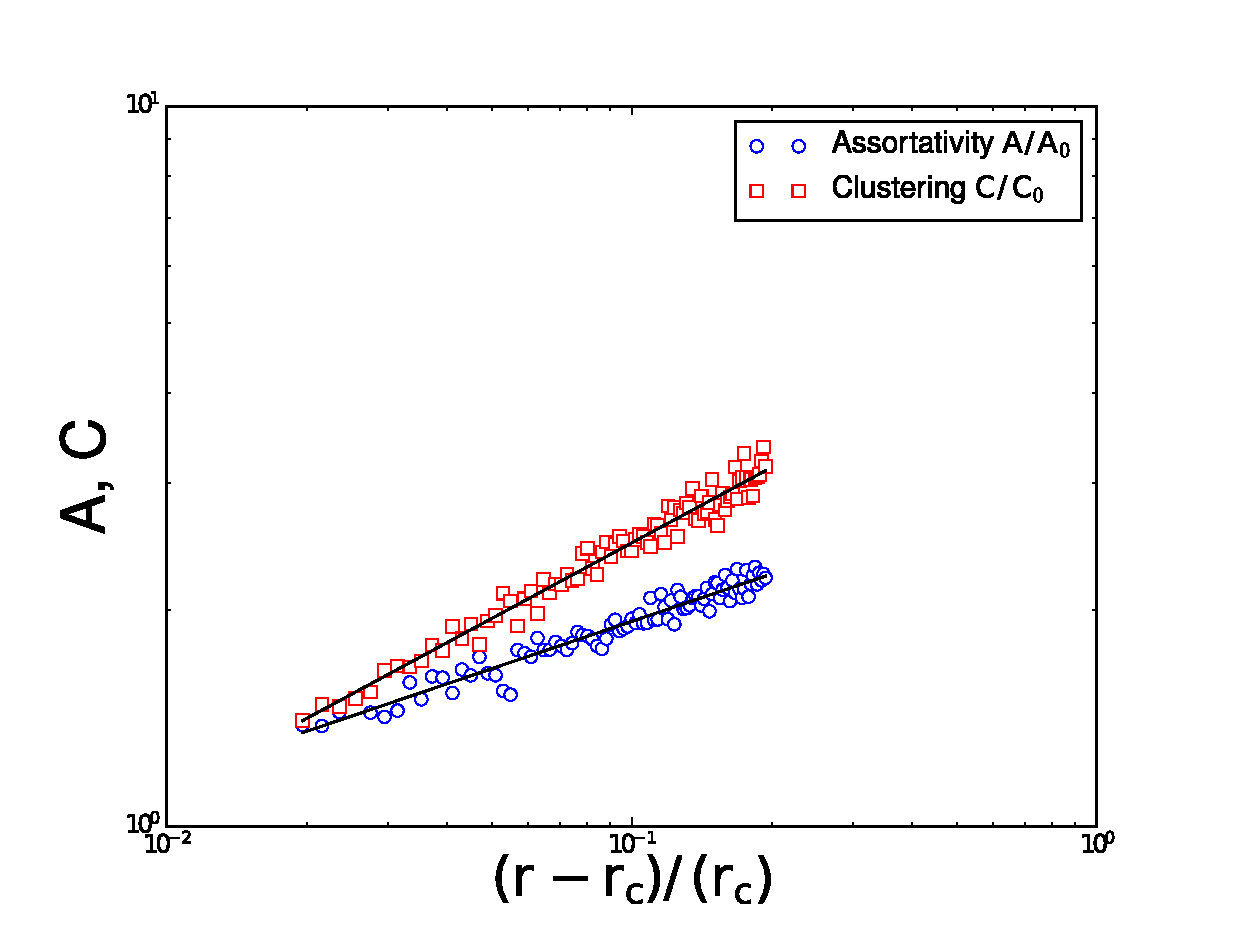
\includegraphics[height=5.5cm]{pygraph/baParamsLog.eps}
}

\caption{
\label{fig:baCharacteristic}
По horizontal axis represents the value of the fault-finding, the vertical axis represents the value of conformance characteristics.
\ subref {fig: baCharacteristic_raw} Change clustering, assortative, the minimum average path when $ r = \ lceil 0,45; 0,56 \ rceil $ steps of 0.01.
\ Subref {fig: rankDistribution_log} Change clustering, assortative, the minimum average path when $ r = \ lceil 0,5; 0,56 \ rceil $ steps of 0.001. In a double-logarithmic
scale.}{figure}
\ End

If $ r \ geq r_c $ this dependence appears, and it is a power, namely $ C \ sim {(r-r_c)} ^ \ alpha $, $ A \ sim { (r-r_c)} ^ \ gamma $, $ l \ sim {(r-r_c)} ^ \ sigma $, where $ \ alpha \ approx 0.46155027 $, $ \ gamma \ approx 0.26025569 $, $ \ sigma \ approx 0.11761072 $ (\ ref {fig:

rankDistribution_log}).%dependence of these characteristics $ (l, C, A, \ eta) $ from $ r-r_c $ is close to apower:%

begin {equation}%\\
\Csim 0.28cdot  ^ {0.543} +  \\{equation}%\\(\ frac {r-r_c} {r_c})
(\{r-r_c}0.039%end
{equation}%begin
frac  {r_c})Asim -0.781cdot -0.258%{equation}%{equation}%{r-r_c} {r_c})^ {equation}
{0.448} \\\(\3.551%\ end
\begin
^ lsim -1.615cdot  frac {0.516}+
end
begin  \\\(\{r-r_c} {r_c}){1.303}2.898%\{equation}%
\{equation}%etasim 472.59cdot  frac  ^  +
end

%The results are approximated by the function $ y \ sim ax ^ b + c $. The phase transition is described by the function $ y \ sim x ^ b $. Thus our approximated function can be written $ \ frac {yc} {a} \ sim x ^ b $. Since we are only interested in the behavior of the function, we can neglect the coefficient $ c $, ie to shift our schedules to the origin. Thus we can write the function is approximated as $ \ frac  y  x ^ b  \{equation}%\\ sim {r-r_c} {r_c})

{1} {a}\$:%begin
simk_1cdot C(\frac  {0.543}%{equation}%{equation}%{r-r_c} {r_c})^ {equation}%{equation
\\\(\\ end  \
\beginbegin
^k_2cdot Asim  frac {0.448}%
end
}%{r_c}){0.516}%{equation}%{equation}%
k_3  l \   ^  \\\ cdot \\ sim (\ frac
\{r-r_c}end
begin
cdotsim (\ frac k_4eta{r- ^ {equation}{The
r_c} {1.303}% end  \

{r_c})\subsection  adjacency matrix for the network with picky}
Consider the adjacency matrix $ A_ {ij} $ for a network with fault-finding. For convenience, the numbering of nodes in the adjacency matrix will lead to the decay of the order of the number of connections. That is $ k_i = \ sum \ limits_ {i} A_ {ij} $ does not increase with increasing $i$.


\begin{figure}[H]  

\centering
\subfigure[]
{
    \label{fig:baRankedMatrix_0}
    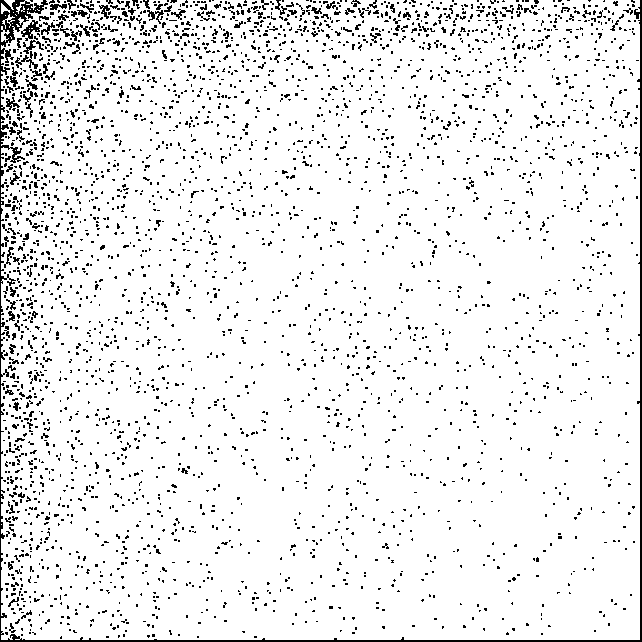
\includegraphics[height=5.5cm]{graphics/bamatrix.png}
}  
\subfigure[]
{
    \label{fig:baRankedMatrix_06}
    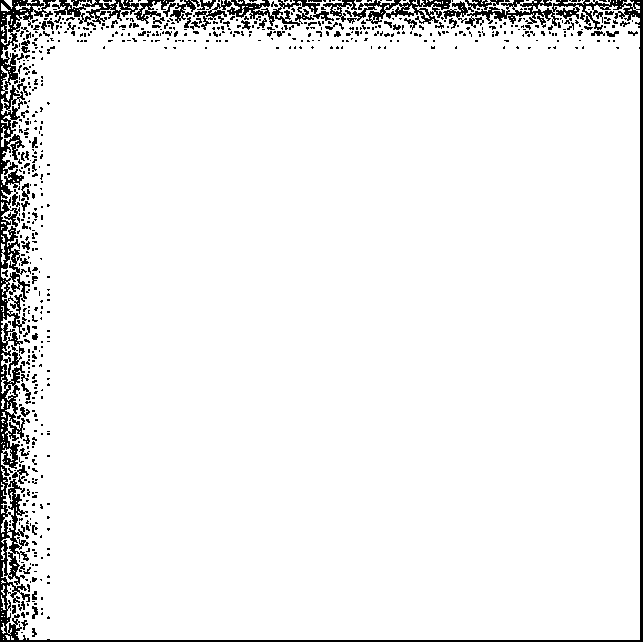
\includegraphics[height=5.5cm]{graphics/bamatrix2.png}
}

\caption{
\label{fig:baRankedMatrix}
Матрица adjacency to a network with $ N = 5000 $ {fig:
nodes:\ subref  baRankedMatrix_0} if $ r = 0.0 $
\ subref {fig: baRankedMatrix_06} if $ r = 0.6
$}{figure}
\ end


The change of the network structure as $ r \ geq r_c $ reflected in the form of adjacency matrix. For a network with $ N = 5000 $ has built two of the adjacency matrix: for $ r <r_c $ - fig. \ Ref {fig: baRankedMatrix_0} for $ r> r_c $ - fig. \ Ref {fig: baRankedMatrix_06}. For udobvstva elements of the adjacency matrix $ A_ {ij} = 1 $ are displayed as a black dot. Both matrices were ranked, ie nodes are numbered in the order of decay of the number of links $ k_i $. Of Fig. \ Ref {fig: baRankedMatrix_06} can be seen that in the adjacency matrix with $ r> r_c $ in the lower right corner of the square there is a large area filled with 0, ie those pairs of nodes that are not connected with each other. This area shows Islenyev experiment in direct proportion depends on the $ r $.

Thus network characteristics such as the clustering coefficient, assortative, the average minimum distance behave like `order parameter '' $  eta $. \

\Section {Hierarchical Network (u, v) -flowers with pridirchiostyu}
In addition to random scale-free networks based on algoritmu Barabshi Alberta (and their generalizations), known for the class of simple determenirovannyh networks are also scale-free networks \ cite {Rozenfeld2} - Fractal and Transfractal Recursive Scale- Free Networks. In particular the so-called (u, v) -flowers, Fig. \ Ref {fig: flowerGraph}.

Below we generalize the model Fractal and Transfractal Recursive Scale-Free Networks, entering the factor `fault-finding '' $ r $ and randomness in the law of network growth. As it turns out in this case, the behavior characteristics of the network is similar to a phase transition.

\ Subsection {Algorithm (u, v) -flowers}
Deterministic growing SF-networks called (u, v) -flowers and (u, v) -trees been proposed and investigated in \cite{Dor1,Rozenfeld1,Rozenfeld2}.

\begin{figure}[H]

\centering
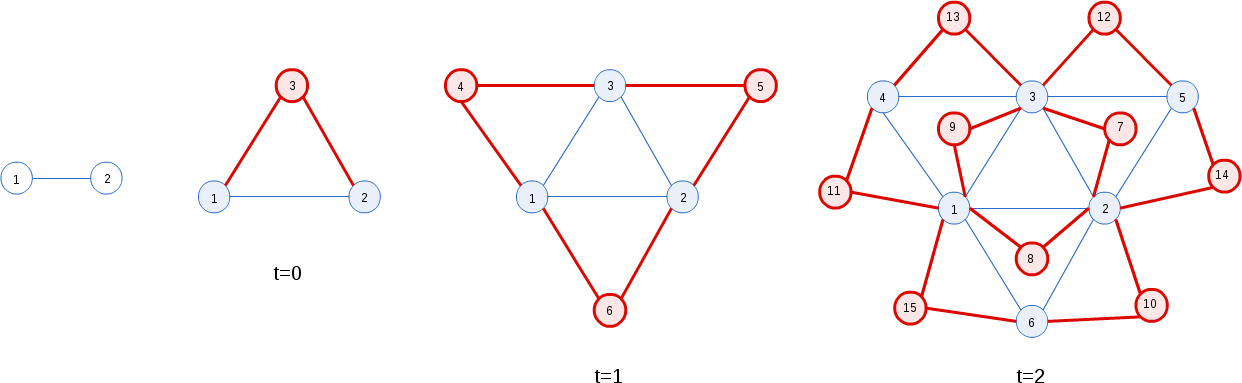
\includegraphics[height=5.5cm]{graphics/hierarhical.png}
\caption{
\label{fig:flowerGraph}
Схема construction of (1,2) -flowers on the steps $ t = 0,1,2 $. Thick (red online) - poyavivschiesya nodes in this step, not thickened (blue online) - nodes that have appeared in the previous {figure}
steps.}\ End

The numbering of nodes in general can be any, but in this example, nodes can be numbered in such a way (see Fig. \ ref {fig: flowerGraph}), that the adjacency matrix $ A_ {ij} $ be the most simple. Under the simple $ A_ {ij} $, we, in this case, we understand its structure such that the largest number of the largest square area $ N \ times N $ in it remain пустыми.


\begin{figure}[H]  

\centering
\subfigure[]
{
    \label{fig:flowerMatrix_real}
    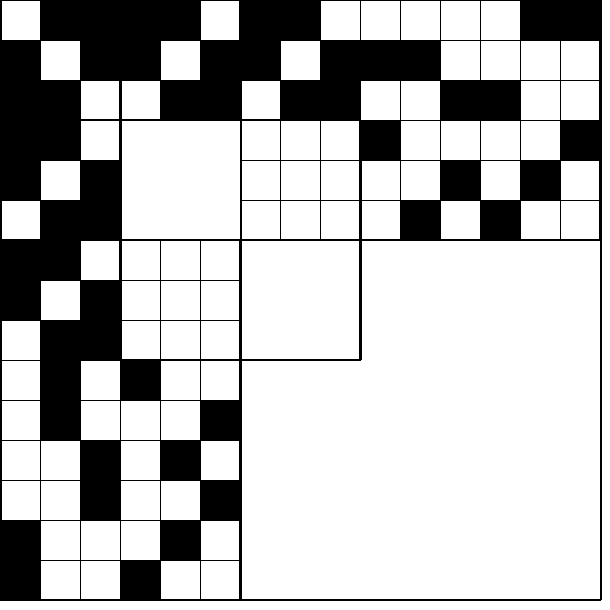
\includegraphics[height=5.5cm]{graphics/first_all.png}
}  
\subfigure[]
{
    \label{fig:flowerMatrix_scheme}
    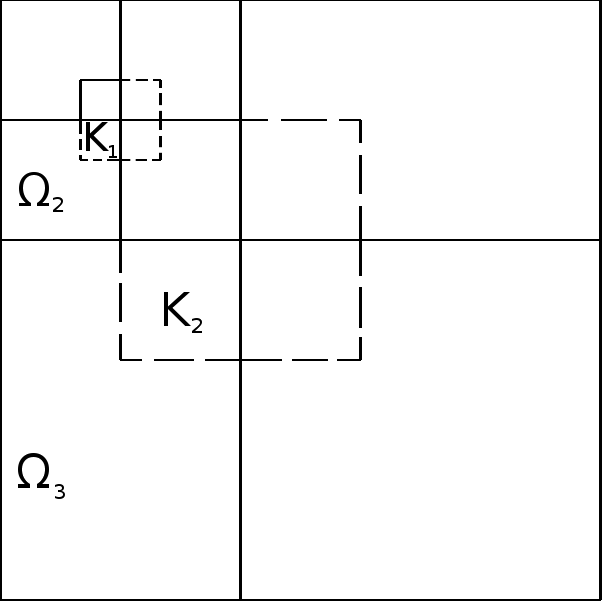
\includegraphics[height=5.5cm]{graphics/second.png}
}

\caption{
\label{fig:flowerMatrix}
Матрицы smezhosti for the third step (1,2) {fig:
-flower:\ subref  baRankedMatrix_0} adjacency matrix of a network with the chosen numbering
\ subref {fig: baRankedMatrix_06} schematic
representation}{figure}
\ end

Figure. \ Ref {fig: flowerMatrix} - $ N \ times N $ adjacency matrix, where black and identify the components of a matrix with $ A_ {ij} = 1 $. In the first step the adjacency matrix $ \ hat {A} $ consists of $ 3 \ times 3 $ elements (top left, step $ t = 0 $ in Fig. \ Ref {fig: flowerGraph}). In the second step, it adds new elements, and the matrix consists of a $ 6 \ times 6 $ elements (step $ t = 1 $ in Fig. \ Ref {fig: flowerGraph}). In the third step step new elements are added, and the matrix consists of a $ 15 \ times 15 $ elements (step $ t = 2 $ in Fig. \ Ref {fig: flowerGraph}). As can be seen from Fig. \ Ref {fig: flowerMatrix} the lower right square of the first step-free connections and consists of a single element. In the second step adds the lower right square, consisting of a $ 3 \ times 3 $ elements, and the third of the $ 9 \ times 9 $ elements. Fig. \ Ref {fig: flowerMatrix} white designated place adjacency matrix, where $ A_ {ij} = 0 $.

When the chosen numbering appear more to the construction of the adjacency matrix in the work \ cite {Dor1} field $ K_1 $, $ K_2 $, in which is also $ A_ {i, j} = 0 $.

At each step $ t $ has $ N_t $ nodes and $ L_t $ Relations  cite  \{equation}\{eq: flowerEdgesNodesRecurent}

\{Rozenfeld1}begin
label
N_t = (u + v) \ cdot N_  - (u + v),  quad L_t = (u + v) ^ t \{equation}
{t-1}\end

Ie at each step $ t $ appears $ N_t-N_ {t-1} $ nodes and $ L_t-L_ {t-1} $ bonds. For example, Fig. \ Ref {fig: flowerGraph}, at step $ t = 1 $ there is 3 knots and 6 ties.

Make the substitution $ (u + v) = w $ and reveal the recurrent formula \ ref {eq: flowerEdgesNodesRecurent} \ cite {Rozenfeld1}:

begin  \{eq: flowerEdgesNodesOpenRecurent}\{w-2}
\{equation}label
N_t =frac  {w-1} \ cdot w ^ t + \ frac {w} {w-1},  quad L_t = w ^ t \
\end {equation}

At each step $ t $ is $ \ Omega_t $ cells, which can be filled - fig. \ Ref {fig: flowerMatrix}. Their number {eq:

\ flowerEmpty}\ begin  \{t}{t-1})
is:\{equation}label
begin {split}
Omega_  & = (N_t-N_  \ cdot N_t-N_ {t-2} ^ 2 = \ frac {w ^ 3-w ^ 2-1} {w ^ 4} N_t ^ 2 + \ frac {w ^ 3-2w ^ 2-2w-2} {w ^ 3} N_t- \ frac {2w ^ 2 + 2w + 1} {w ^ 2} = \\
           & = \ Frac {w ^ {2t + 4} -5w ^ {2t + 3} + 8w ^ {2t + 2} -5w ^ {2t + 1} + 4w ^ {2t} + w ^ {t + 5} -3w ^ {t + 4} + 4w ^ {t + 2} -w ^ 5} {w ^ {3} \ cdot (w-1) ^2}{split}{equation}
\ end
\ end

The probability of filling the cell matrix равна:

\begin{equation}
W_t=\frac{L_t-L_{t-1}}{\Omega_t}=\frac{w^{t+5}-3w^{t+4}+3w^{t+3}-w^{t+2}}{w^{2t+4}-5w^{2t+3}+8w^{2t+2}-5w^{2t+1}+4w^{2t}+w^{t+5}-3w^{t+4}+4w^{t+2}-w^5}
\end{equation}

Так c each step the probability decreases and the adjacency matrix becomes more and more depleted.
In \ cite {Dor1} it was shown that (u, v) -flowers are scale-free networks. To the one shown in Fig. \ Ref {fig: flowerGraph} (1,2) -flower distribution of nodes in powers of the form $ P (k) \ sim k ^ {- (1+ \ frac {\ ln {3}} {\ ln {2}} )} $. In the general case  -flowers  cite  \{equation}(k)\{-\  \\\{\{(u

\{Rozenfeld1}begin
(u, v)P sim k ^ alpha},quadalpha = 1+fracln+ v)}} {\ ln {equation}
{2}} end  \{A

\subsection  modification of the algorithm (u, v) -flowers}

We now consider the situation where the construction of (u, v) -flower not all links are implemented. At what probability unrealized connection is greater than is less than the degree of the nodes it соединяет.

\begin{figure}[H]

\centering
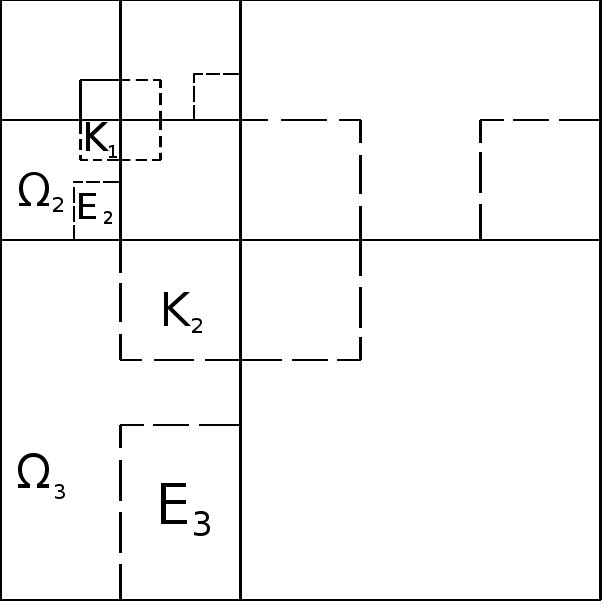
\includegraphics[height=5.5cm]{graphics/third_n.png}
\caption{
\label{fig:flowerMatrixExceptive}
Схема smezhosti matrix for the third step (1,2) {figure}
-flower.}\ end

The computer simulation was carried out by filling in the adjacency matrix domains $ \ Omega_1, \ Omega_2 ... $ sootetsvuyuschim them with the number of ties $ L_t $. Thus `fault-finding 'in the adjacency matrix is shown right bottom corners of regions $ \ Omega $. When $ r> 0 $ in the lower right corners of fields $ \ Omega $ Blank areas appear. In our simulations, we used the empty field $ E_t $ \ ref {fig: flowerMatrix}. Then the probability of filling the cell матрицы:

\begin{equation}
W_t=\frac{L_t-L_{t-1}}{\Omega_t-E_t}
\end{equation}

\begin{equation}
E_t= (R \ cdot N_ {t-1}) \ times (r \ cdot (N_t - N_ {equation}
{t-1})) end  \{The

\subsection  distribution function of the degrees of nodes}

When the value of fault-finding $ r = 0 $ The proposed model takes the form of a standard (u, v) -flowers. As is the case with the model Barabasi-Albert model (u, v) -flowers present threshold parameter faultfinding $ r_c $. When the parameter is less than a certain threshold faultfinding $ r <r_c $ node degree distribution function $ P (k) $ is a power, and the network itself, thus, scale-free network. При значениях параметра придирчивости больше порогового значения $r \geq r_c$ сеть меняет свою структуру.

Определим пороговое значение параметра придирчивости. Для этого рассчитаем пороговое значение для (u,v)-flowers с 1 по 14 поколение, при этом будем усреднять значения по 50 экспериментам. Как и в модели Барабаши-Альберт с придирчивостью происходит насыщение порогового значения. Для 9 поколения $r_c$ полностью насыщается и мы получаем $r_c=0.6$. Необходимо отметить, что при $r>=0.6$ происходит изменение структуры и характеристик сети, однако видимый разрыв появляеться при $r>=0.8$, что мы можем увидеть на рис. \ref{fig:flowerRank_08}


\begin{figure}[H]  

\centering
\subfigure[]
{
    \label{fig:flowerRank_06}
    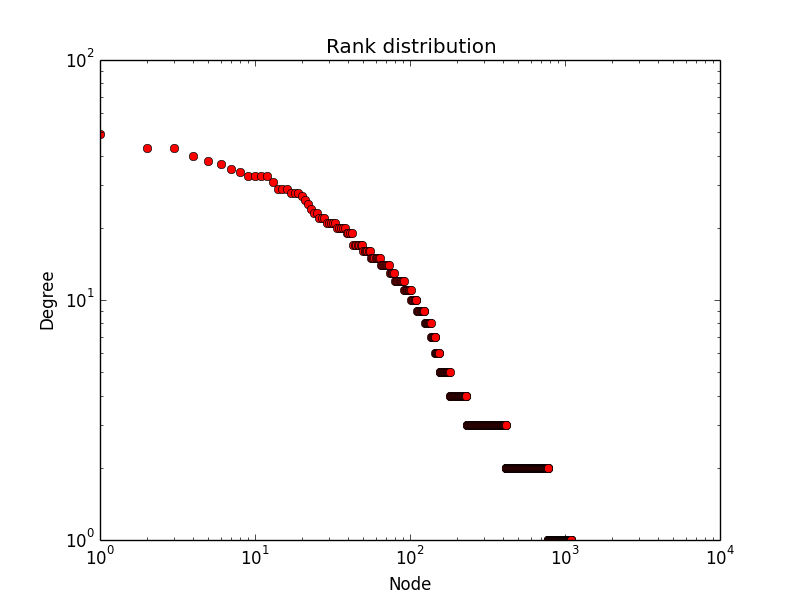
\includegraphics[height=4cm]{graphics/flowerDecor6.png}
}  
\subfigure[]
{
    \label{fig:flowerRank_08}
    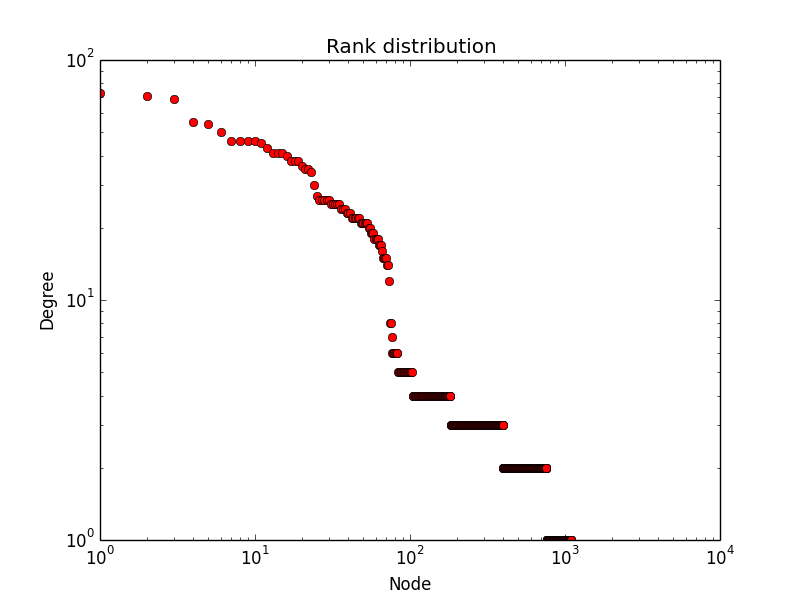
\includegraphics[height=4cm]{graphics/flowerDecor8.png}
}
\subfigure[]
{
    \label{fig:flowerRank_gap}
    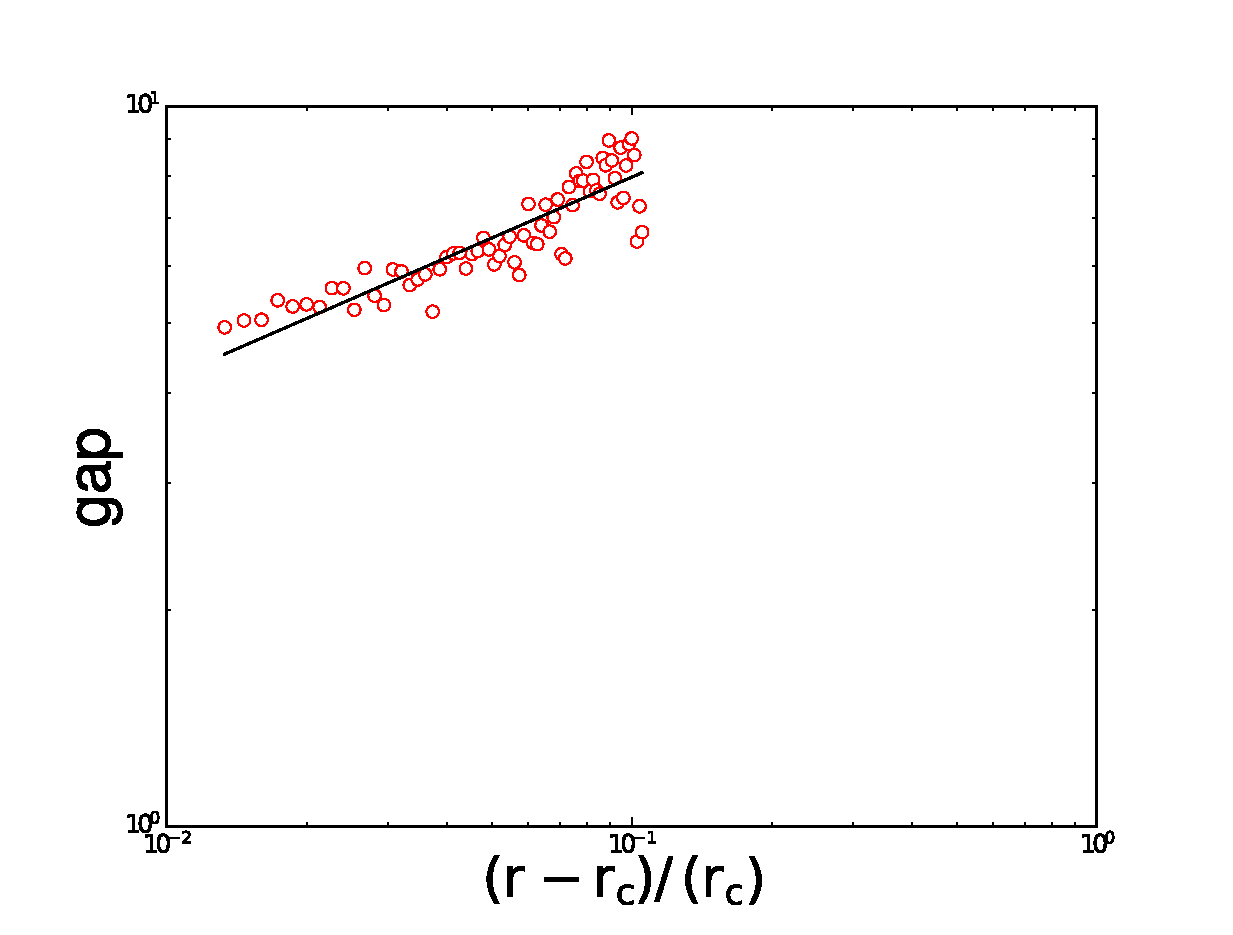
\includegraphics[height=4cm]{pygraph/flowerGap.eps}
}

\caption{
\label{fig:flowerRank}
\subref{fig:flowerRank_06} Ранжированое распределение сети при $r=0.6$. По горизонтальной оси отложено порядковый номер узла, по вертикальной оси отложена степень узла.
\subref{fig:flowerRank_08} Ранжированое распределение сети при $r=0.8$. По горизонтальной оси отложено порядковый номер узла, по вертикальной оси отложена степень узла.
\subref{fig:flowerRank_gap} Величина разрыва при увеличении $r$ от $r_c$ до $r_c + 0.2$ с шагом $0.01$. По горизонтальной оси отложено $\frac{r-r_c}{r_c}$, по вертикальной оси отложено значение величины разрыва.
}
\end{figure}

Как следует из численного моделирования, поведение параметра $\eta$ аналогично поведению параметра порядка в теории фазовых переходов второго рода \cite{Landau}. Параметр порядка $\eta$ при приближении к критическому значению уменьшается степенным образом $\eta \sim (r-r_c)^\beta$, где $\beta$ – критический индекс.
При проведении численного эксперимента были выбраны следующие начальные параметры: (1,2)-flowers седьмого поколения, тоесть количество узлов $N=1095$.

На рис. \ref{fig:flowerRank_gap} показана полученная зависимость $\eta = A \cdot {(r-r_c)}^\beta$, где $\beta \sim $

\subsection{Коэфициент кластеризации, ассортативность, минимальное среднее расстояние, величина разрыва}
Ниже рассмотрено поведение $C$ - коэффициента кластеризации, $A$ - ассортативности и $l$ - минимального среднего расстояния, как функции коэффициента придирчивости $r$, при $r \geq r_c$. Как показал численный эксперимент для сети (1,2)-flowers седьмого поколения с $N=1095$ узлов, коэфициент кластеризации $C$, ассортативность $A$, минимальное среднее расстояние $l$ при $r<r_c$ от $r$ не зависит и равна $C_0 \approx 0.02$, $l_0 \approx 4.05$, $A_0 \approx -0.18$, что, как и должно быть, совпадает с расчетами приведенными в \cite{Rozenfeld1,Rozenfeld2}.

При увеличении $r$ от $r_c$ до $r_c + 0.1$ с шагом $0.01$ коэффициент кластеризации увеличивается от $0.02$ до $0.04$, ассортативность уменьшается от $-0.18$ до $-0.39$, среднее минимальное расстояние уменьшается от $4.0$ до $3.65$(согласно рис. \ref{fig:flowerParam_raw}). Для нормализации зависимости возьмем отношение параметра к его значению при $r<r_c$, а также приведем зависимости к возрастающим функциям: $A=\frac{A}{A_0}$, $C=\frac{C}{C_0}$, $l=-\frac{l}{l_0}$.

\begin{figure}[H]  

\centering
\subfigure[]
{
    \label{fig:flowerParam_raw}
    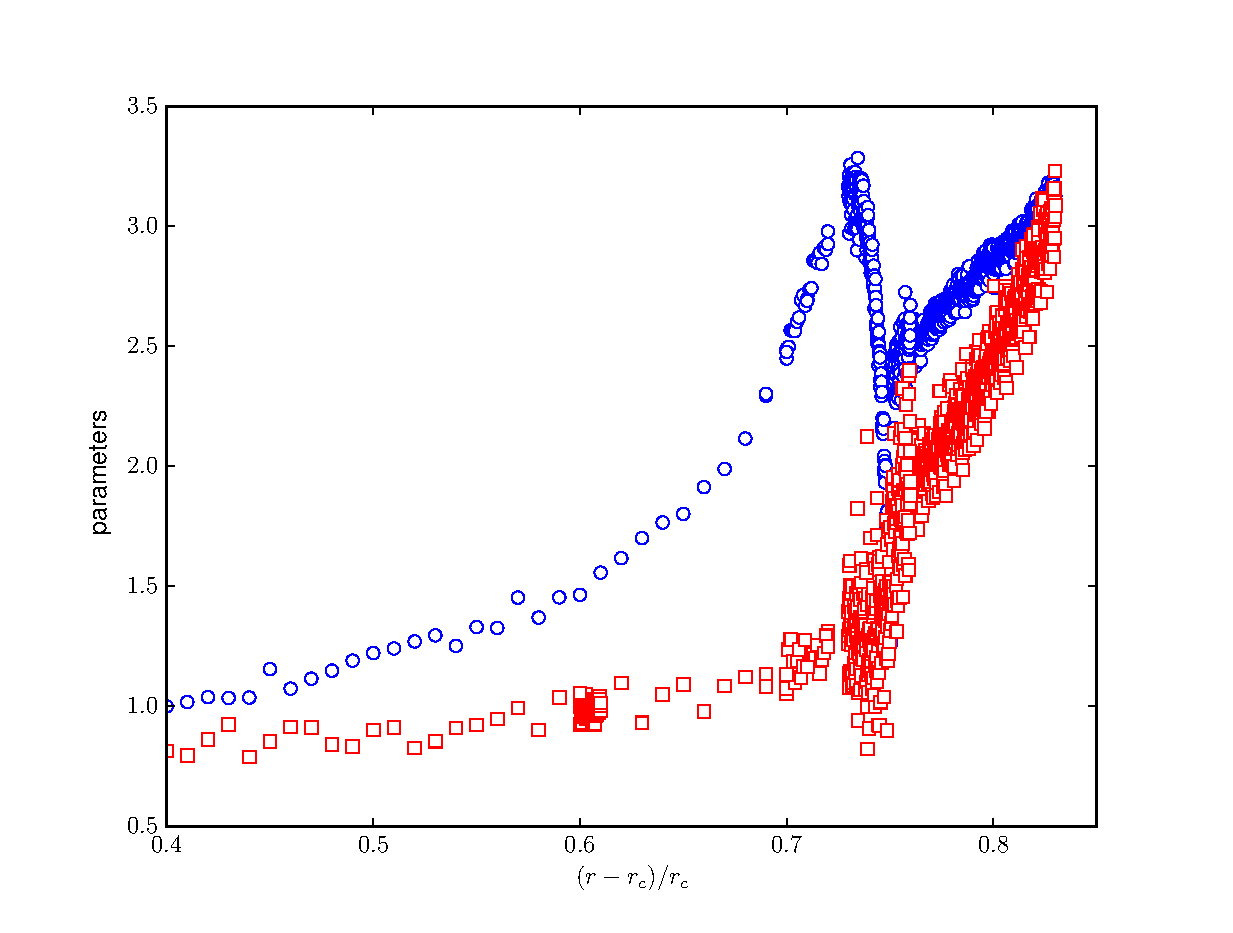
\includegraphics[height=5.5cm]{pygraph/flowerParams.eps}
}  
\subfigure[]
{
    \label{fig:flowerParam_log}
    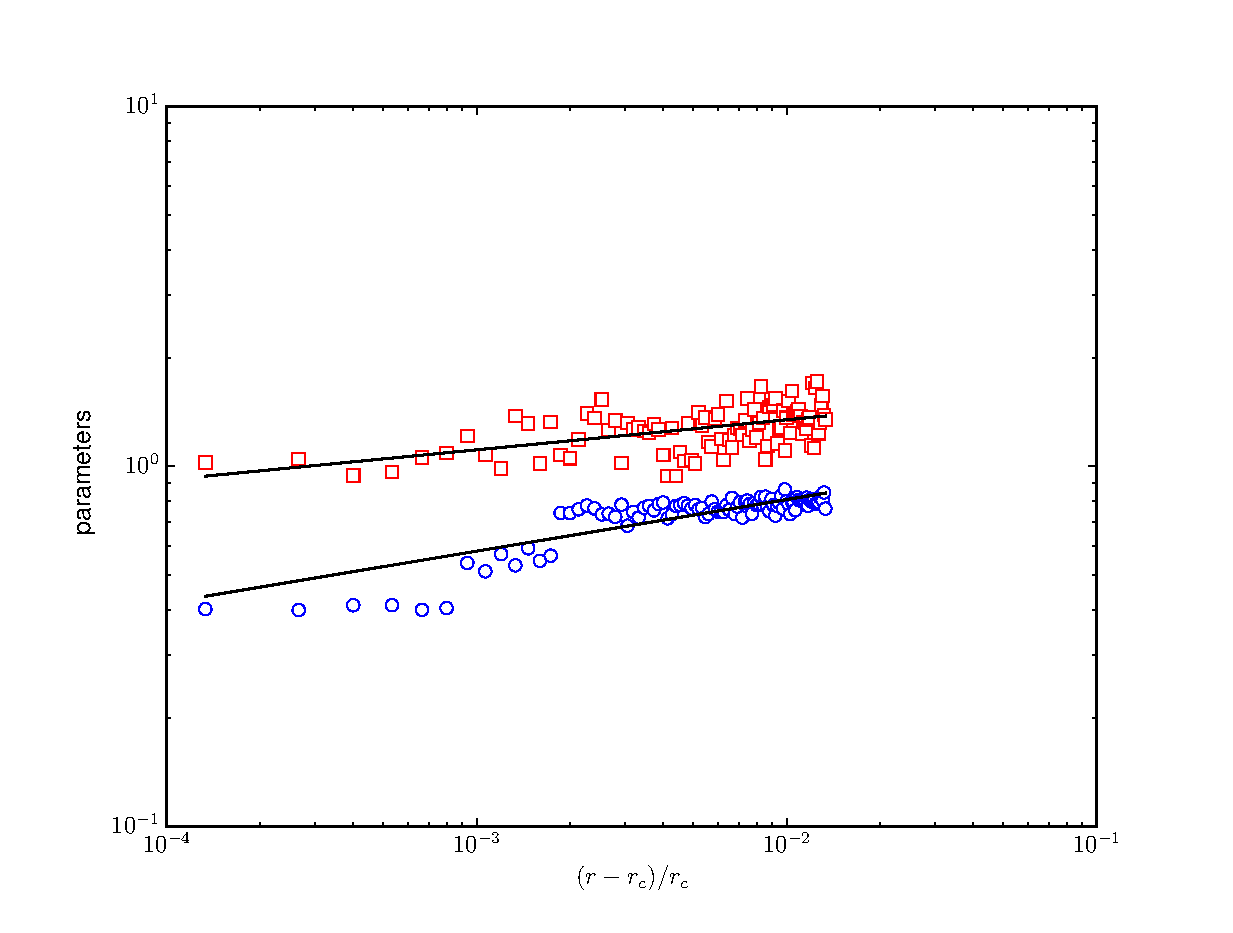
\includegraphics[height=5.5cm]{pygraph/flowerParamsLog.eps}
}

\caption{
\label{fig:flowerParam}
По горизонтальной оси отложено значение параметра придирчивости, по вертикальной оси отложено значение соответсвующей характеристики.
\subref{fig:baCharacteristic_raw} Изменение кластеризации,ассортативности, минимального среднего пути при $r=\lceil 0,4; 0,72 \rceil$ с шагом 0.01.
\subref{fig:rankDistribution_log} Изменение кластеризации,ассортативности, минимального среднего пути при $r=\lceil 0,59; 0,7 \rceil$ с шагом 0.001. В двойном логарифмическом масштабе.
}
\end{figure}

При $r \geq r_c$ такая зависимость появляется, и она оказывается степенной, а именно $C \sim {(r-r_c)}^\alpha$, $A \sim {(r-r_c)}^\gamma$, $l \sim {(r-r_c)}^\sigma$, где $\alpha \approx 0.11379367$, $\gamma \approx 0.43169254$, $\sigma \approx 0.01796628$ (\ref{fig:flowerParam_log}).

% \begin{equation}
% k_1 \cdot C \sim (\frac{r-r_c}{r_c})^{1.216}
% \end{equation}
% \begin{equation}
% k_2 \cdot A \sim (\frac{r-r_c}{r_c})^{0.963}
% \end{equation}
% \begin{equation}
% k_3 \cdot l \sim (\frac{r-r_c}{r_c})^{0.817}
% \end{equation}
% \begin{equation}
% k_4 \cdot \eta \sim (\frac{r-r_c}{r_c})^{0.256}
% \end{equation}

\section{Заключение}

Обычно заключение отвечает на три вопроса:
Что за проблема решалась в статье?
Какие результаты были получены в статье?
Ну и что!?
Для ответа на эти вопросы, в особенности на последний, хорошо поиграть в игру Ну и что?!. То есть представьте, что вы беседуете с редактором журнала, и он вас спрашивает: ну и что в статье интересного-то?" или почему я должен обратить на это внимание?.

Показано что матрица смежности

!!!!!!!!!Что-то про р, параметр придирчивости

В результате исследования было предложено новое правило предпочтительного соединения, которое значительно меняет структуру сложной сети: в ранжированном распределении степеней узлов появляется существенный разрыв. Данный результат был получен путем введения в правило предпочтительного соединения параметра ``придирчивости''. В качестве новой характеристики сети была введена величина разрыва. В статье было изучено поведение разрыва и основных характеристик предложенной модели, которое можно описать как фазовый переход второго рода. Также было показано влияние параметра ``придирчивости'' на матрицу смежности.

Полученные результаты возможно применить для построения экономических моделей.
!!!!!!!!Что-то про економическую часть.

\section{Литература}

\bibliographystyle{plain}
\bibliography{biblio}

\end{document}


